\documentclass{../../myassignment}

\usepackage{array}

\courselabel{IN1030}
\exercisesheet{Oblig 2}{Bruk og brukerundersøkelser}

\usepackage{xcolor}
\definecolor{block-gray}{gray}{0.85}

\usepackage{environ}

\NewEnviron{myblock}
{\colorbox{block-gray}{%
\parbox{\dimexpr\linewidth-2\fboxsep\relax}{%
\small\addtolength{\leftskip}{5mm}
\addtolength{\rightskip}{5mm}
\BODY}}
}

\renewcommand{\quote}{\myblock}
\renewcommand{\endquote}{\endmyblock}

\begin{document}
	\subsection*{Oppgave 1 --- Observasjon av bruk}
	\paragraph*{a)}

	% Planlegg datainnsamlingen. Beskriv følgende:
		% Hva du forventer å finne ut ved å studere interaksjonen mellom en bruker og den digitale løsningen, og hvem du tror faller innenfor målgruppen til systemet?
		Ved {\aa} studere interaksjonen mellom flere brukere av det eksisterende Vy-systemet og dens maskiner forventer jeg {\aa} finne ut hvordan folk generelt sett tiln{\ae}rmer seg en togstasjon. Jeg har allerede opplevd selv at problemer allerede kan oppst{\aa} f{\o}r vi engang n{\aa}r det digitale punktet. Eksempler inkluderer at vi ikke vet hvor stedet ligger, ikke finner inngangen, eller ikke kjenner igjen maskinene. 

		I noen omstendigheter vet ikke brukeren om protokollene heller, og det finnes ingen lett tilgjenglige instrukser. Forskjellige aldersgrupper og forskjellige bakgrunner vil ha forskjellige problemer, og m{\aa}ter {\aa} l{\o}se disse problemene p{\aa}. Jeg {\o}nsker {\aa} f{\aa} et innblikk i disse grupperingene, og finne frem generiske l{\o}sninger og betraktninger man m{\aa} tenke p{\aa}.

		% Opp til 5 relevante oppgaver du vil be deltakeren om å utføre i systemet.
		\begin{itemize}
		\item[---] Kj{\o}pe en billett via datamaskin. 
		\item[---] Kj{\o}pe en billett ved en vilk{\aa}rlig og ukjent stasjon. 
		\item[---] Refundere en billett.
		\item[---] Finne frem fra en stasjon til en annen stasjon, uten aa bruke eksterne hjelpemidler (alts{\aa} ved {\aa} bare bruke Vy-tilbudte systemer). 
		\item[---] F{\aa} kontakt med en ansatt for {\aa} sp{\o}rre etter hjelp (toalettet? spr{\aa}khjelp? assistanse? {\dots}?)
		\end{itemize}


		% Deltakeren. Er hun/han en del av målgruppener
		Deltakeren jeg har valgt er en del av den yngre m{\aa}lgruppen. Yngre mennesker er en del av fremtiden, og burde kanskje derfor bli prioritert n{\aa}r det gjelder innovasjon, men p{\aa} den andre siden s{\aa} er det gjerne de yngre gruppene som trenger minst hjelp. Det beste ville v{\ae}rt {\aa} sp{\o}rre flere ``typer'' mennesker, og f{\aa} et bredt innblikk av systemet. {\AA} ha muligheten til {\aa} gj{\o}re denne observasjonen i utlandet gir meg muligheten til {\aa} observere hvordan systemet fungerer her, for {\aa} s{\aa} sammenligne med systemet i Norge, og eventuelt se forskjellen mellom hvordan folk oppf{\o}rer seg annerledes her enn der.

		% Din relasjon til deltakeren. Hvordan tror du dette kan spille inn på dataen du samler inn?
		Siden jeg er ganske kjent med dev vedkommende deltageren ville det kanskje v{\ae}re lett {\aa} tenke seg at jeg vil forvrenge resultatene av observasjonen, men jeg er ganske vant med {\aa} v{\ae}re ekstern observat{\o}r uten {\aa} innblande meg. Desutten vil jeg informere om dette f{\o}r observasjonen, for {\aa} unng{\aa} innblanding.

		% Hvordan du vil registrere data under observasjonen, som for eksempel medpenn/papir, opptak av lyd, fotografier, video, annet?
		Jeg har tenkt {\aa} forklare gj{\o}rem{\aa}lene hver for seg, og filme diverse snutter som jeg videre analyserer hjemme. Jeg tror det vil v{\ae}re lettere {\aa} analysere detaljer i etterkant ved {\aa} kunne se ting om igjen, med god tid. Alternativet ville v{\ae}rt {\aa} skrive ting opp etterhvert som de skjer, eller bare bruke hukommelsen. Om deltageren ikke {\o}nsker {\aa} bli filmet vil jeg forbrede handligssekvens-tabellen i forkant, for {\aa} s{\aa} skrive fortl{\o}pende det jeg ser. 

		Konklusjonen og utdypelsen av analysen m{\aa} skje i etterkant uansett, men ikke alt for lenge etter, siden hukommelsen ogs{\aa} har et betydning i helheten.


	\newpage

	\paragraph*{b)}

	Personvern er en viktig del av integriteten til alle og enhver. {\AA} vite hvilken informasjon av en selv som blir brukt av andre er viktig for mange, og fra et filosofisk standspunkt ville det ver uetisk {\aa} bruke informasjon om andre uten deres modne, fullverdige, og frie sammtykelse. 

	Det er i tillegg p{\aa}krevd av alle land innenfor EU {\aa} f{\o}lge GDPR (General Data Protection Regulation), p{\aa}krevd siden 2018 med bakgrunn p{\aa} etiske prinsipper som tidligere ble brutt. {\AA} ikke f{\o}lge denne loven kan risikere selskapet store p{\aa}legg, og eventuelt bli lagt ned om ledelsen ikke tilrettelegger l{\o}sninger, og f{\o}lger disse.

	\paragraph*{c)}

	\begin{quote}
		Sammtykelse for student-observasjon\\

		Jeg, Christian Burja, godtar, forst{\aa}r, og samtykker med at mitt navn blir registrert i en del av unders{\o}kelsen som ble gjort den 20. februar i 2020. Om ønsket kan jeg bli kontaktet for utdypende spørsmål i etterkant via mail \texttt{cburja@gmail.com} Denne informasjonen vil bli brukt til akademiske form{\aa}l som en del av en student-unders{\o}kelse, og vil ikke bli behandlet i en komersiell sammenheng. I tillegg vet jeg at jeg har mulighet til å trekke meg fra denne undersøkelsen ved å kontakte observatøren, og dermed fjerne den personlige informasjonen som er brukt og lagret om meg. 

		Ved {\aa} signerere dette dokumentet lar jeg Rolf Vidar Mazunki Hoksaas observere og ta opp det jeg gj{\o}r, for {\aa} videre analysere situasjonen, valgene, og omheng. Resultatene av observasjonen vil kunne bli publisert via Universitet i Oslo, eller via observatørens personlige platformer, enten med, eller uten mitt navn. Dette gj{\o}r jeg av min egen fri vilje, uten noen personlig gevinst, eller noen form for press. 



	\end{quote}


	\paragraph*{d)}
	I og med at jeg har gjort en observasjon på en bruker allerede i første innlevering av denne obligen, vil dette fungere som en pilotundersøkelse, i en større grad en å gjøre pilotundersøkelsen på meg selv. Det er lettere å se etter problemer når man kan få ekstern tilbakemelding på hvordan det opplevdes å være deltaker i observasjonen. 

	Det største ``problemet'' brukeren opplevde med den forrige interaksjonen var unødvendig/uvanlig kjøp av billetter, siden formålet med interaksjonen var å simulere en faktisk situasjon. Det er ikke alltid like lett å finne en bruker som skal bruke systemet allerede, men i en ekte observasjon ville man kunne be tilfeldige kunder om å bli observert når vi ser dem tilnærme seg maskinene, eller benytte seg av et testing-system. I og med at dette kun er en akademisk simulasjon blir ting litt annerledes en det ville vært i en ekte observasjon. Jeg er selv vant med å bruke test-modus på Ruter-maskiner for å bli kjent med systemet, så jeg vet at dette er en nyttig, effektiv og lett måte å løse slike problemer på. 

	Ellers var det muligvis en litt dårlig struktur mellom da vi faktisk gikk gjennom de forskjellige punktene av ting å gjennomføre i pilotundersøkelsen, selv om det var enklere å observere hvordan brukeren benyttet systemet når jeg som observatør holdt meg til siden uten å innblande meg.

	\newpage
	\paragraph*{e)}
	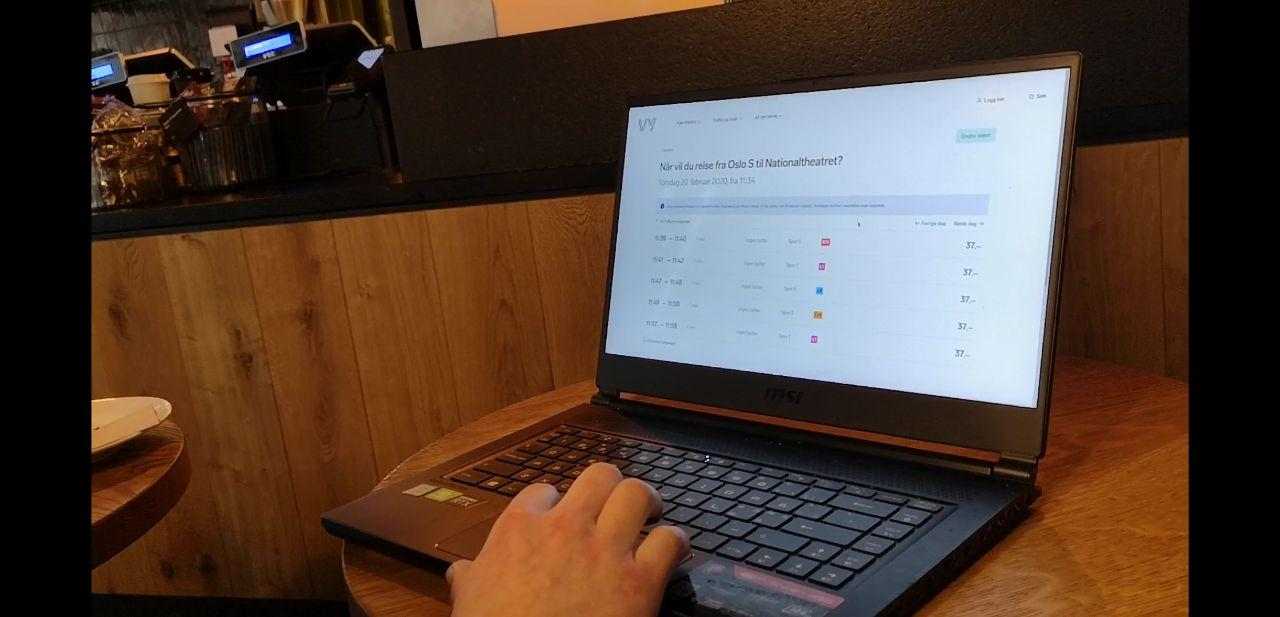
\includegraphics[scale=0.25]{pictures2/traveltimes.jpg}

	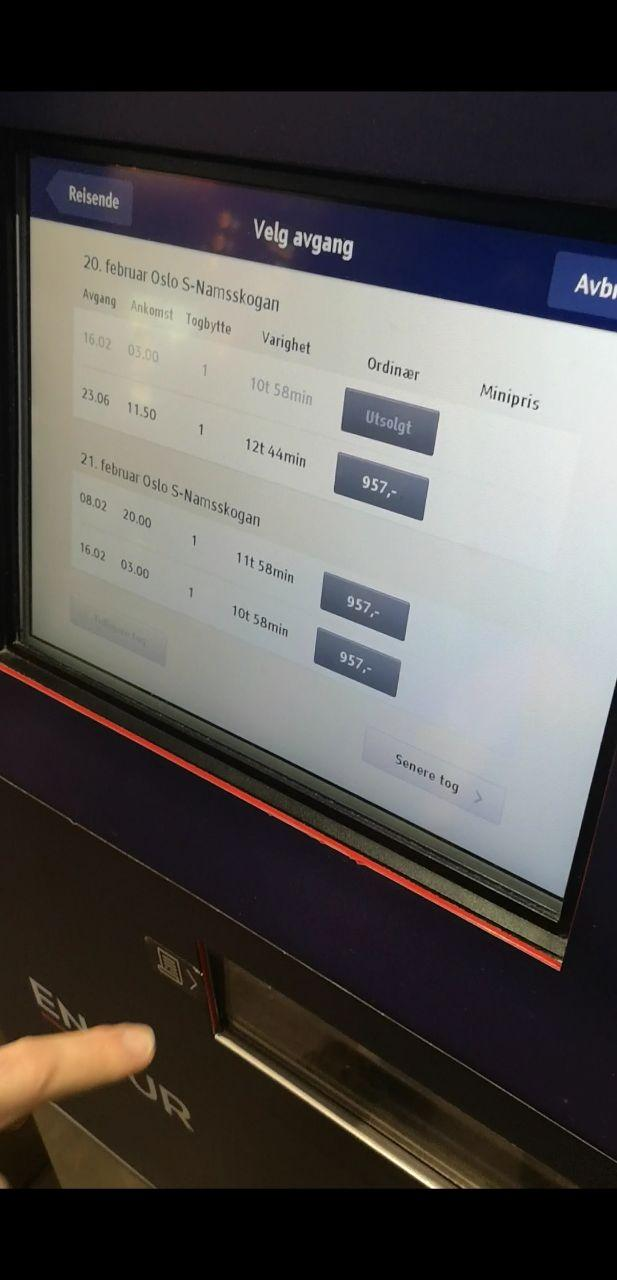
\includegraphics[scale=0.25]{pictures2/departureprices.jpg}
	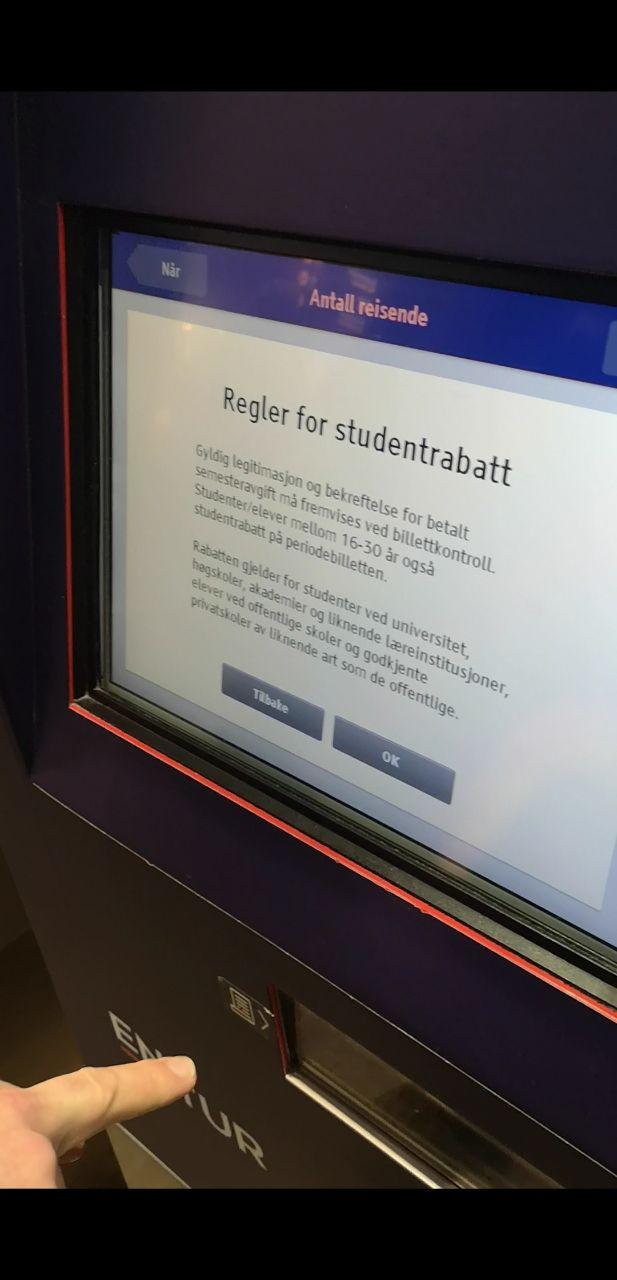
\includegraphics[scale=0.25]{pictures2/studentdiscount.jpg}
	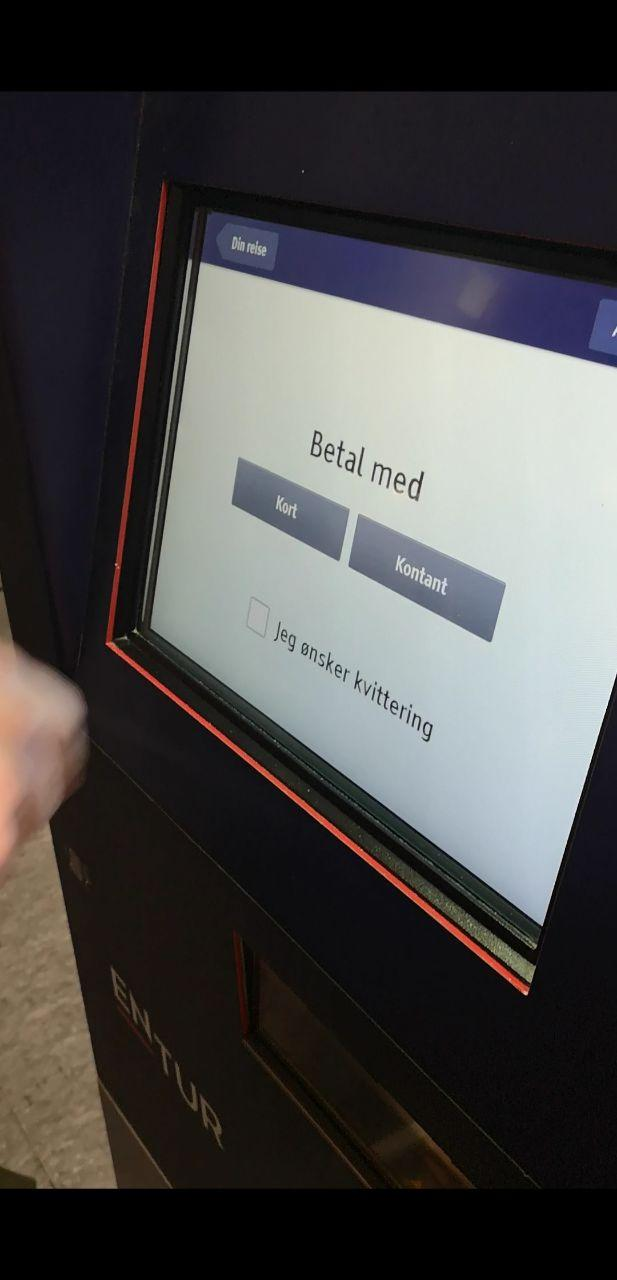
\includegraphics[scale=0.25]{pictures2/paywith.jpg}

	
\includegraphics[scale=0.25]{pictures2/transaction.jpg}
	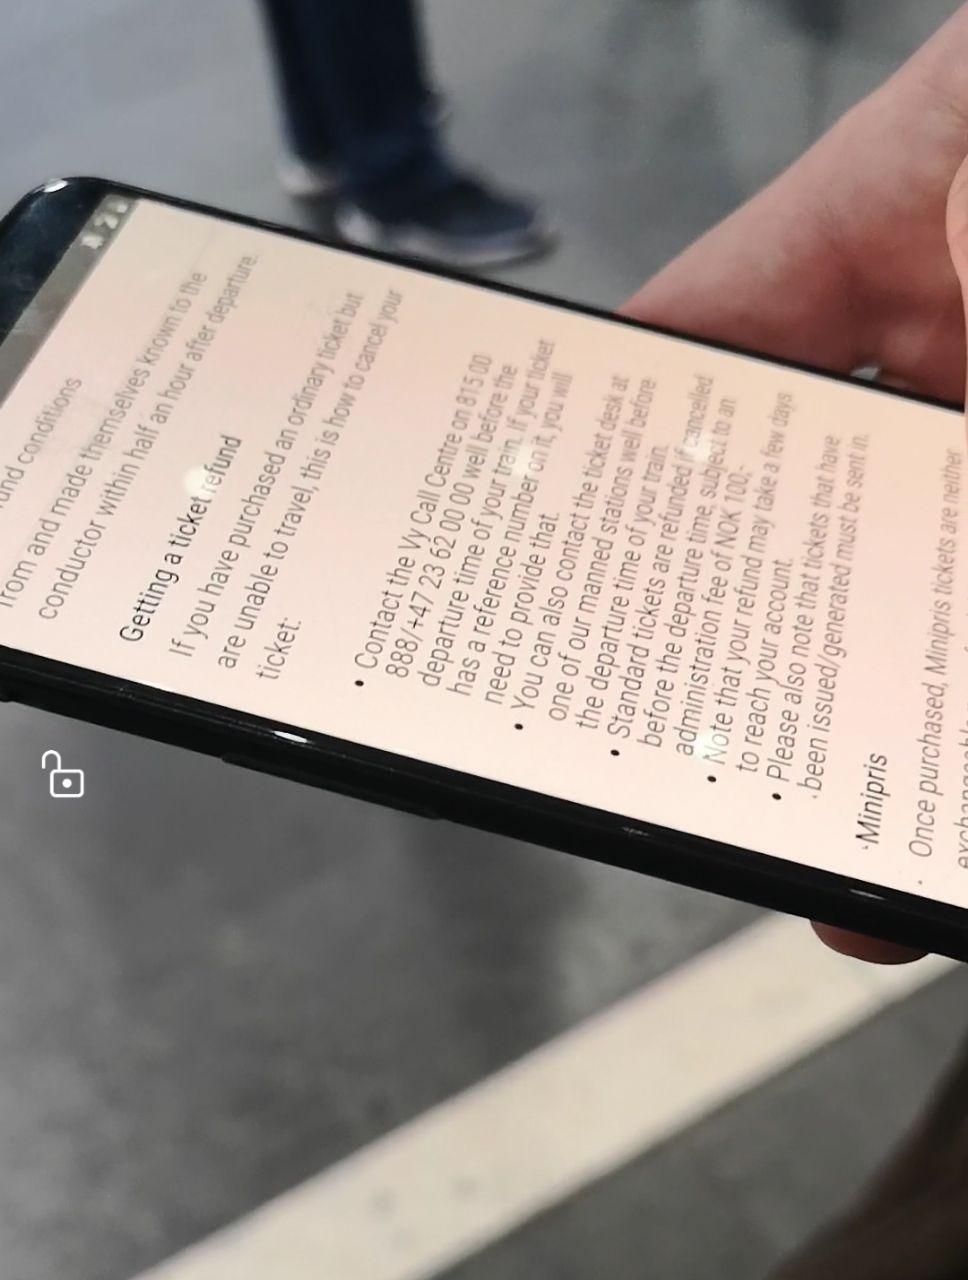
\includegraphics[scale=0.25]{pictures2/refundconditions.jpg}

	\newpage

	\subsection*{Oppgave 2 --- Analyse: Sekvens av handlinger}
	\paragraph*{a)}
	En handlingsekvenstabell er en ``to-dimensjonell''-tabell som beskriver hvordan en bruker og en maskin kommuniserer. Langs ``y-aksen'' har vi tidsrommet, og langs ``x-aksen'' har vi i grunnen to spalter, som igjen er hver delt i to.

	Til venstre har vi brukeren, og til h{\o}yre har vi maskinen. Ytterlig til venstre fremkommer alt brukeren gj{\o}r som ikke maskinen ser, og tilsvarende ytterlig til h{\o}yre fremst{\aa}r det maskinen gj{\o}r i bakgrunnen. I de to gjenst{\aa}ende spaltene i midten ser vi hva brukeren og maskinen sier til hverandre. Vi kan rapportere om miljøet rundt brukeren i den første kolonnen, og hvordan vi antar eller vet at systemet fungerer i den siste kolonnen. I kolonnene i mellom ser vi den fysiske interaksjonen mellom bruker og maskin.

	I de ytterlige kolonnene er mye informasjon, som muligvis er viktig {\aa} formidle til hverandre.

	Form{\aa}let med denne type tabell er \aa{} kunne analysere hvordan brukere interagerer med maskiner. Vi vil kunne se hvilke forst{\aa}else-problemer som finnes i systemet, for {\aa} dermed ha mulighet til {\aa} forbedre disse.

	\newpage

	\paragraph*{b)}  % tabell

	\begin{tabular}{ | >{\centering}p{10em} || >{\raggedleft}p{10em} | >{\raggedright}p{10em} || >{\centering\arraybackslash}p{10em} | }
	\hline
	\multicolumn{2}{|c|}{Human} & \multicolumn{2}{c|}{Machine} \\\hline
	Environment & {To Machine} & To Human & System design\\\hline\hline
	Wanders around looking at different machines & & & \\\hline
	Notices a machine saying EnTur &  & & \\\hline
	Looks around for Vy machine &  & & \\\hline
	Assumes EnTur is Vy &  & & \\\hline
	Says loudly ``This must be the same!'' &  & & \\\hline
	 & Presses one of the machines & & \\\hline
	 & Tries to search for Nationaltheateret, but presses wrong station & & \\\hline
	Gets confused at price & & & Says nothing about the selected option\\\hline
	 & Presses return & & \\\hline
	 & Does the same mistake, again & & \\\hline
	 & Chooses 1 student & & \\\hline
	 &  & Informs about Student criteria & \\\hline
	 & Presses next & Informs about what the ticket is valid for & Assumes user knows ``train'' means ``Vy train'' \\\hline
	Expects to see more info while pressing next & Presses pay & & \\\hline
	 & Returns & & \\\hline
	 & Goes next & & \\\hline
	Is scared ticket is not valid & Pays & & \\\hline
	Complains about ticket not saying what companies it is valid for &  & & \\\hline
	Complains about ticket not being refundable &  & & \\\hline
	Looks for customer agent &  & & \\\hline
	Quickly sees one &  & & \\\hline
	Customer agent helps user after being asked &  & & \\\hline
	& & & Ticket is valid for Vy \\\hline
	\end{tabular}

	\paragraph*{c)}  % analyse av tabell

	Interaksjonen med maskinen er lett s{\aa} lenge man vet hva en gj{\o}r, hva en {\o}nsker, og hvordan systemet fungerer. Hvis ikke man vet hvilken billett man {\o}nsker, og ``bare gj{\o}r det'', oppst{\aa}r det forvirrelser. Det er ikke lett å vite om billetten faktisk hører til Vy eller ei, man må bare anta at det vil fungerere. Dette problemet oppstår ikke om man betaler online.

	Det er enkelt nok å spørre etter hjelp til et menneske på dagtid, men på natten er det kanskje ikke like enkelt, eller hvis brukeren ikke tør å spørre fremmede etter hjelp. Hadde maskinene hatt logoen av Vy på seg ville dette problemet ikke eksistert. Siden man ikke kan refundere billetten, i utgangspunktet, og det koster 100 kroner å be etter en refundering er dette dårlig butikk om man har gjort en feil ved å ikke kjenne systemet. Problemer oppstår gjerne oftere når man er stresset, og det er nemlig da vi minst ønsker dem (siden det skaper enda mer stress, og vi har dårlig tid).

	\subsection*{Oppgave 3 --- Øvelse: Oppmerksomhet og distraksjon}

	{\AA} skru av telefonen/nettet er noe jeg er ganske vant med. Jeg bruker telefonen, datamisknen, og b{\ae}rbaren aktivt nesten hver dag for tiden, men (nesten) aldri n{\aa}r jeg er p{\aa} jobb. Hvis noen ringer meg p{\aa} jobben s{\aa} svarer jeg bare dersom det er sjefen, eller andre viktige jobb-kontakter. Hvis ikke det er noen jeg har aktivt lagt til i unntakene til ``Do Not Disturb''-moduset vil jeg ikke f{\aa} notifkasjon f{\o}r etter jeg har tid til {\aa} sjekke meldingene. Jeg anbefaller alle {\aa} ta seg tid til {\aa} sette opp telefonen(e) sine for {\aa} bare f{\aa} de meldingene de er interessert i, og ikke alt annet tull. Tross alt, er det er din telefon, og ikke du som er telefonen sin. 

	{\AA} bruke telefonen som et verkt{\o}y er en positiv ting, s{\aa} lenge man ikke er avhengig av denne. Skru gjerne av telefonen i flere uker om du f{\o}ler den tar kontroll over livet/hverdagen din, siden det betyr at det har g{\aa}tt for langt. Det er fullt mulig {\aa} leve uten telefon selv i dag, der alle andre forventer deg til {\aa} f{\o}lge med p{\aa} lasset. Det handler bare om {\aa} tilpasse seg, ha selvkontroll, og v{\ae}re bevisst om hva en driver med. 

	\subsection*{Oppgave 4 --- Spørsmål til pensum}

	\begin{itemize}
		\item[---] Har det v{\ae}rt noen endring gjennom historien relatert til hva folk foretrekker mellom ``objektive'' og ``ekspressive'' statistikker/m{\aa}linger?
		\item[---] Trenger vi {\aa} m{\aa}le ting objektivt for {\aa} komme til konklusjoner, eller er det nok {\aa} f{\o}lge ``bobler'' som kunstig intelligens kan vise oss?
		\item[---] Kan vi relatere forskjellige m{\aa}leteknikker til forskjellige typer intellgense? Vil noen mennesker ha det lettere for {\aa} forst{\aa} ting om vi presenterer informasjon p{\aa} en ``strippet'' og ``tall-orientert'' m{\aa}te enn andre? 
	\end{itemize}

	\subsection*{Oppgave 5 --- Refleksjon}

	Den mest informative delen ved denne obligen var delen om m{\aa}linger. Jeg tenker ofte p{\aa} forskjellige m{\aa}ter {\aa} ``lese og skrive'' informasjon, s{\aa} jeg synes det er spennende {\aa} l{\ae}re om forskjellige m{\aa}ter man kan presentere eller samle samme informasjonen/virkeligheten. Likevel synes jeg det var spennende {\aa} gj{\o}re observasjonsdelen, selv om jeg ikke f{\o}lte jeg observerte nok deltagere for {\aa} f{\aa} noe generell informasjon om hvordan brukere generelt anvender systemet. Jeg tror det ville v{\ae}rt mer effektiv {\aa} gj{\o}re en eller flere sp{\o}rreunders{\o}kelser.

	{\AA} kunne sammenligne systemet her i Barcelona versus systemet i Norge tror jeg har v{\ae}rt den  mest nyttige delen ang{\aa}ende forskjellige systemet, siden jeg merker forskjellen p{\aa} hvordan folk bruker systemene her med tanke p{\aa} hvordan disse er lagt opp. Jeg tror ogs{\aa} at {\o}konomien og kulturen definerer hvordan systemene m{\aa} v{\ae}re for {\aa} v{\ae}re effektive. Det finnes intet perfekt system som fungerer overalt. Systemene m{\aa} tilpasses folket der det blir brukt.

\end{document}